\section{Simulation of the Shunt Active Filter Operating with an Electrohidraulic Actuator}

A simulation is proposed to evaluate the shunt active filter operating in an aircraft electrical system. The system is composed by the generation and distribution system and some loads constituted by electrohydraulic actuators with shunt active filter connected to its respective inputs.

\subsection{Active Filter Model}

The shunt active filter model is composed by the current reference calculator and the compensator blocks. The reference calculator block is given by the procedure which uses the instantaneous power theory to define the proper reference to be applied in the compensator input. The compensator block consists of a voltage source converter (VSC), with its respective capacitor DC voltage regulated by a closed-loop controller. The compensator also has the hysteresis controller which creates the commands that are applied in the VSC switching devices.

The active filter operation requires a passive capacitor filter applied in the transmission lines to eliminate the high frequency content injected in the system by the switching commutation \cite{}. As the switching commutation is set at high frequency, this passive filter might be lightweight and does not impact significantly in the aircraft system. However, the presence of capacitors in the transmission lines may decrease the power factor due to current phase shift. To eliminate this problem some inductor may be applied in the lines to compensate the reactive power flow.

The shunt active filter diagram is presented in Fig. \ref{fig:filtro_blocos.png}. This figure shows the blocks where each calculation step is accomplished, and the points where the active filter with its respective voltage and current measurement probes are connected to the electrical grid.

\begin{figure*}[!tb] %
	\centering
	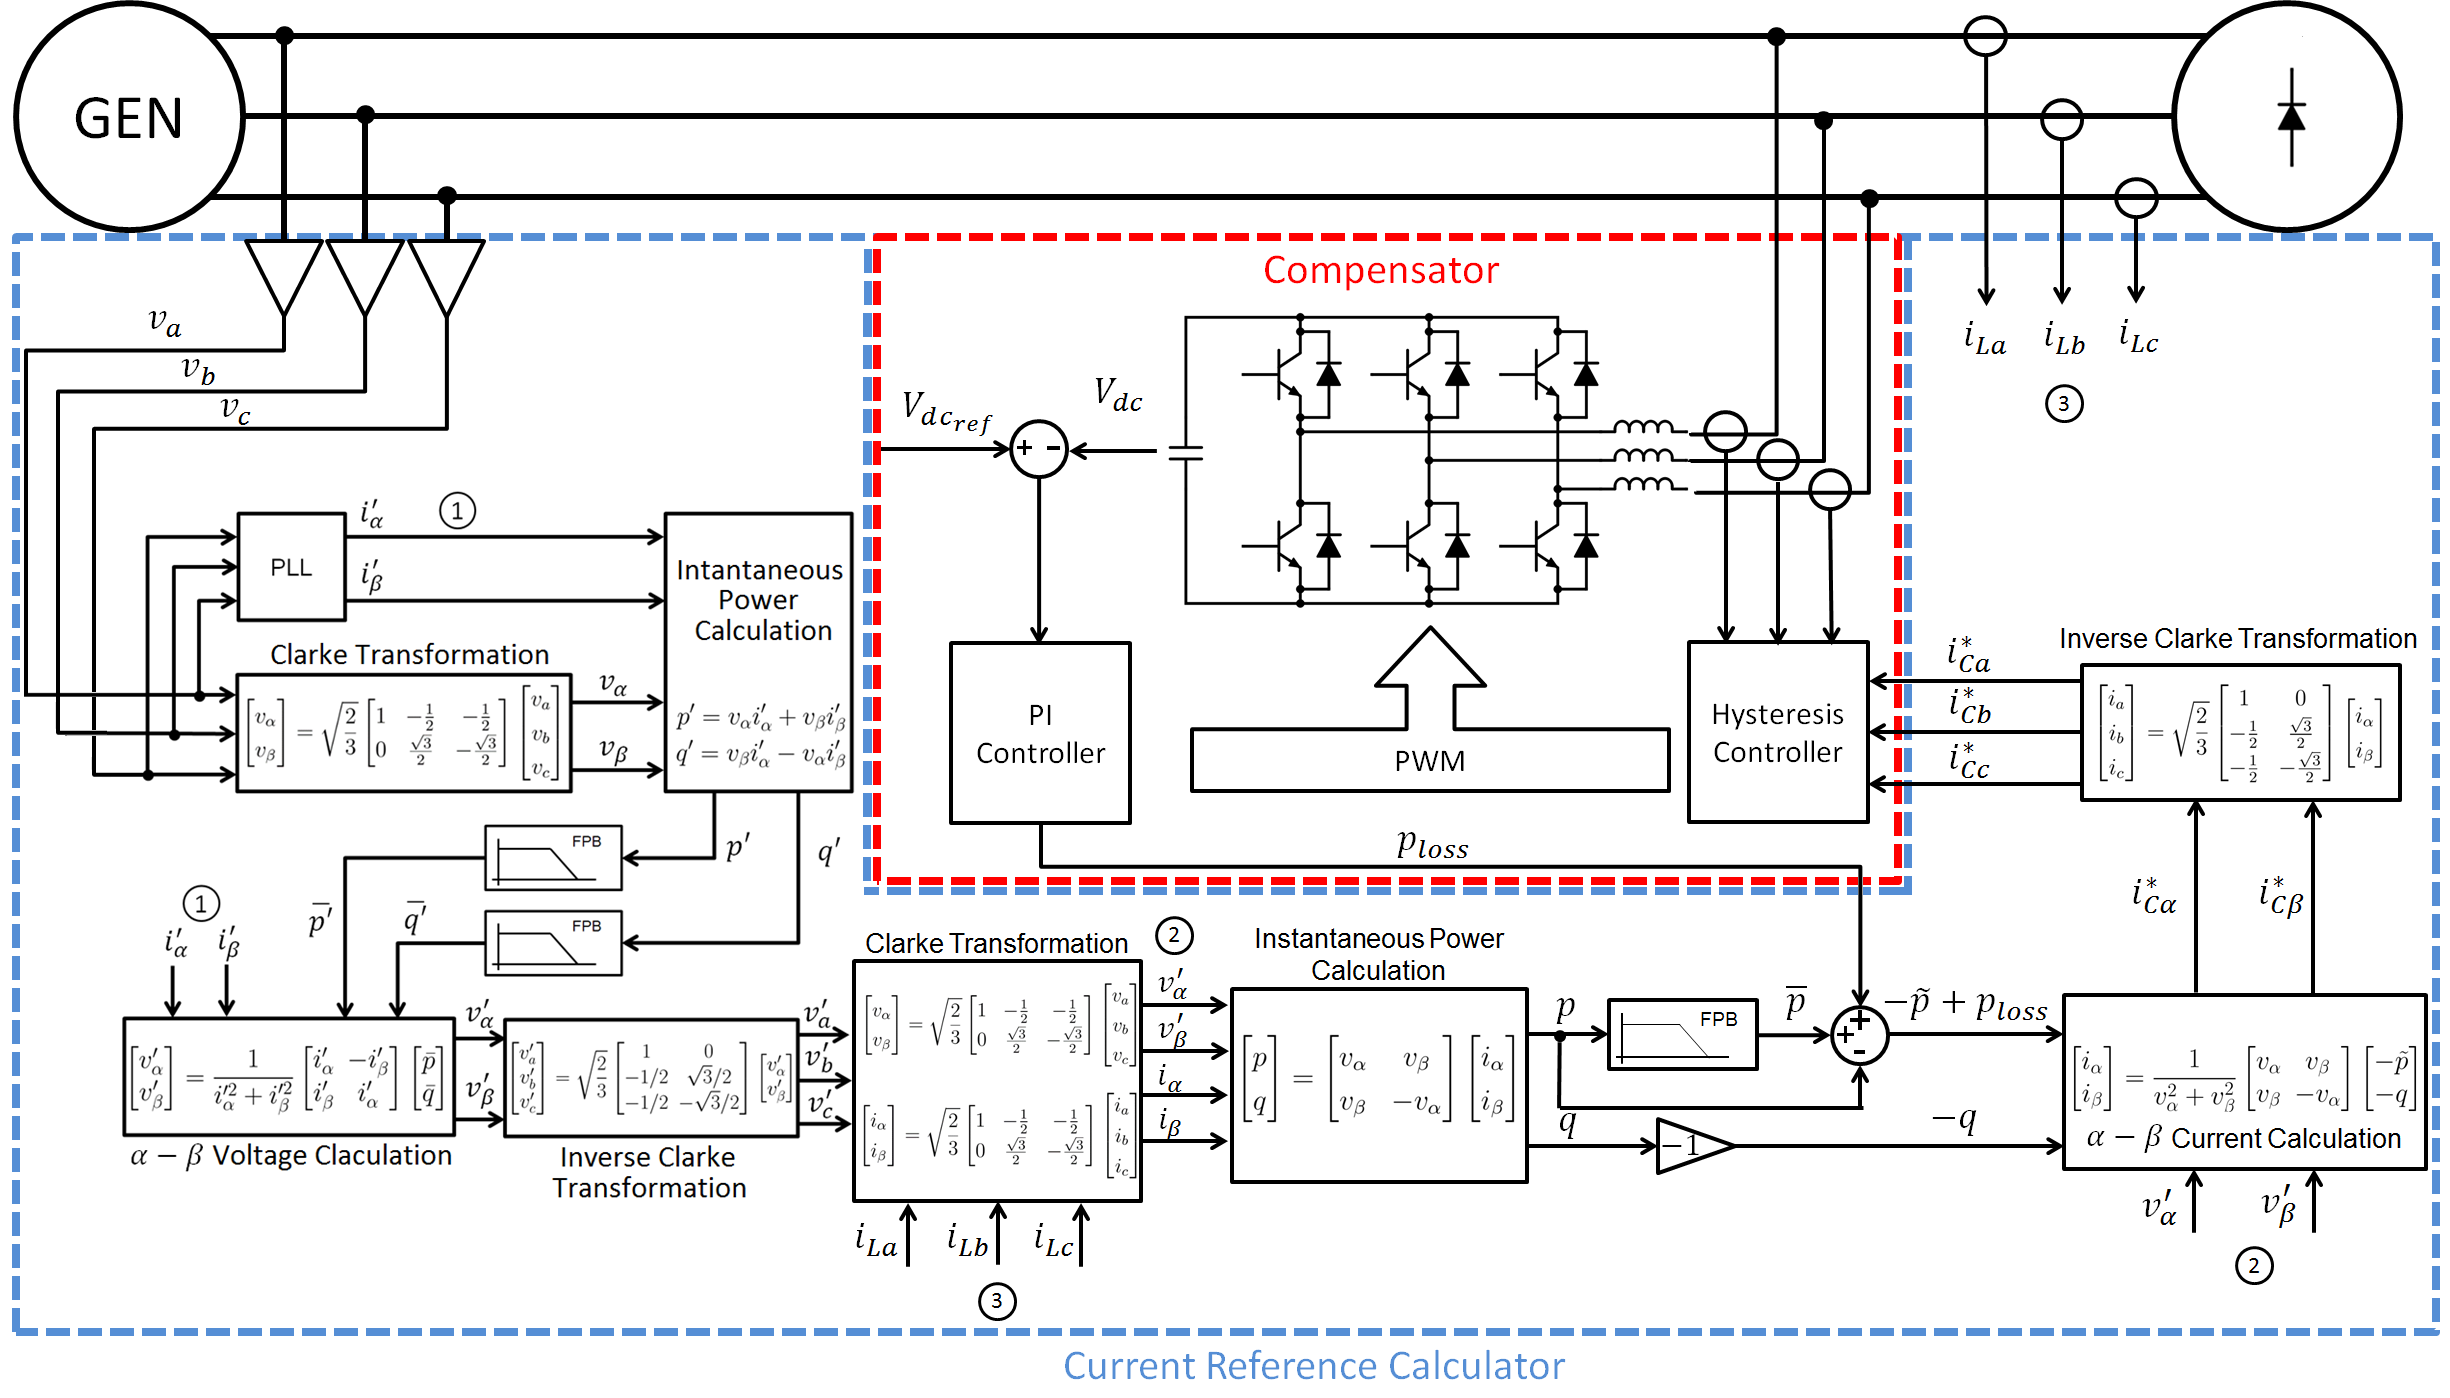
\includegraphics[width=0.8\textwidth]{Figures/filtro_blocos.png}
	\caption{Shunt active filter scheme}
	\label{fig:filtro_blocos.png}
\end{figure*}

\subsection{Electrical System Model}

The aircraft electrical system was modeled based on the operation of the generation and distribution system, with it respective non-idealities, which affect the power quality due to voltage drop. The simulation presents a generator system, a power distribution system and three EHAs connected in parallel as a load, as shown in Fig. \ref{fig:simulacao_simulink.png}.

The generator system is compound of a synchronous machine and a generator control unit (GCU). The GCU works as a field excitation controller to set the proper voltage in the PCC. The synchronous machine also has resistive and inductive reactance connected in series with the voltage source to model the resistance and the inductance presented in the generator coils.

The power distribution system is composed by the transmission lines between the generator and the PCC and between the PCC and EHAs. In the PCC, it is located the probes which measure the system voltages levels to be sent as the reference input to the GCU. The power transmission lines are modeled as resistive and inductive reactance in series for each 3 phase lines.

The EHA is an equipment used in the aircraft aerodynamic surfaces for latero-directional and longitudinal control. This equipment is a non-linear load, since in its input has a 3-phase diode bridge. The EHAs modeled has a 3 phase Graetz diode bridge with a current controlled source placed in its respective DC side. The controlled current source is defined to operate in such way to recreates the apparent power consumption of a real EHA. Thereby, this guarantees the application of the distorted current waveforms generated by the EHA in real operation.

\begin{figure*}[!tb] %
	\centering
	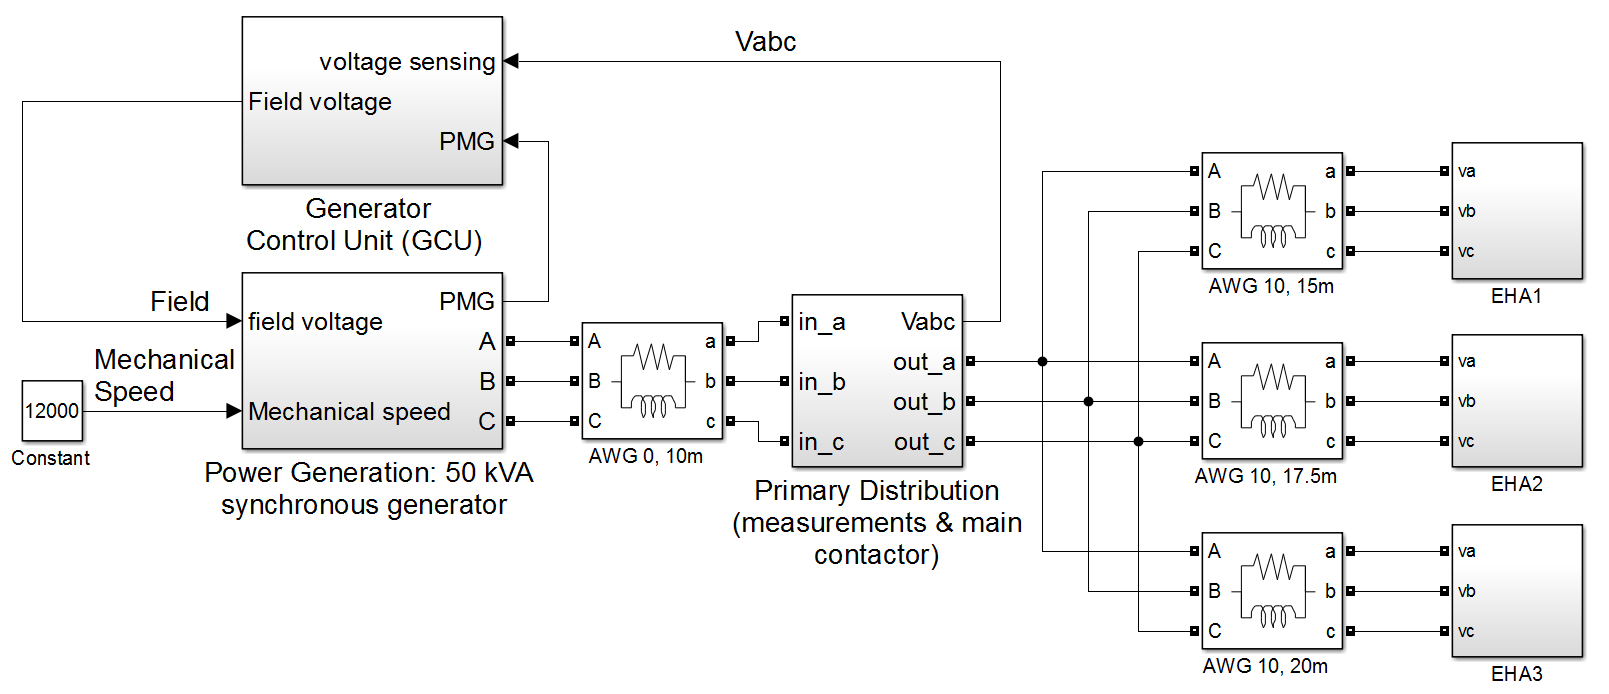
\includegraphics[width=0.6\textwidth]{Figures/simulacao_simulink.png}
	\caption{Electrical generation and distribution model}
	\label{fig:simulacao_simulink.png}
\end{figure*}

\subsection{Results}

The results obtained by the simulation of the system are presented below. These results show the voltages and currents waveforms measured in the PCC, as well as the frequency spectrum with the amplitude limits defined by the MIL-STD 704F together with the calculated value of the voltage THD and IHC.

The test is divide in two portions: The first part is given with the EHAs not requiring any load, and the second part is given when EHAs are starting their operation, where it is observed the maximum load consumption. The results also show the cases where the active filters are connected and disconnected from the EHAs power input.

For the portion where the EHAs are not operating, Fig. \ref{fig:artigo_unfilt_1.eps} and Fig. \ref{fig:artigo_unfilt_2.eps} show the waveforms when the system has no active filters operating. For the same period, Fig. \ref{fig:artigo_filt_1.eps} and Fig. \ref{fig:artigo_filt_2.eps} show the waveforms when the active filters are connected in the EHAs power input. For this interval, the presence of the active filters degrades the power quality, since the THD increase and the frequency spectrum presents more harmonic content. This noise is inserted in the system due to the commutation of the VSC switching devices. Thus, even with the presence of the capacitor filter in the lines, it was observed some high frequency content injected in the grid. However, despite of this adversity, the results are still inside the limits defined by aeronautical standards.

For the portion where the EHA is requiring maximum load, Fig. \ref{fig:artigo_unfilt_3.eps} and Fig. \ref{fig:artigo_unfilt_4.eps} show the waveform when the active filters are not connected in the grid. In this period, Fig. \ref{fig:artigo_filt_3.eps} and Fig. \ref{fig:artigo_filt_4.eps} show the waveforms when the active filters are connected in the EHAs power input. In this interval, it is clear the enhancement that the active filter implies in the system power quality. Considering these results, the active filters operate to mitigate the harmonic content and set it inside the limits of the MIL-STD 704F.


\begin{figure}[!h] %
	\centering
	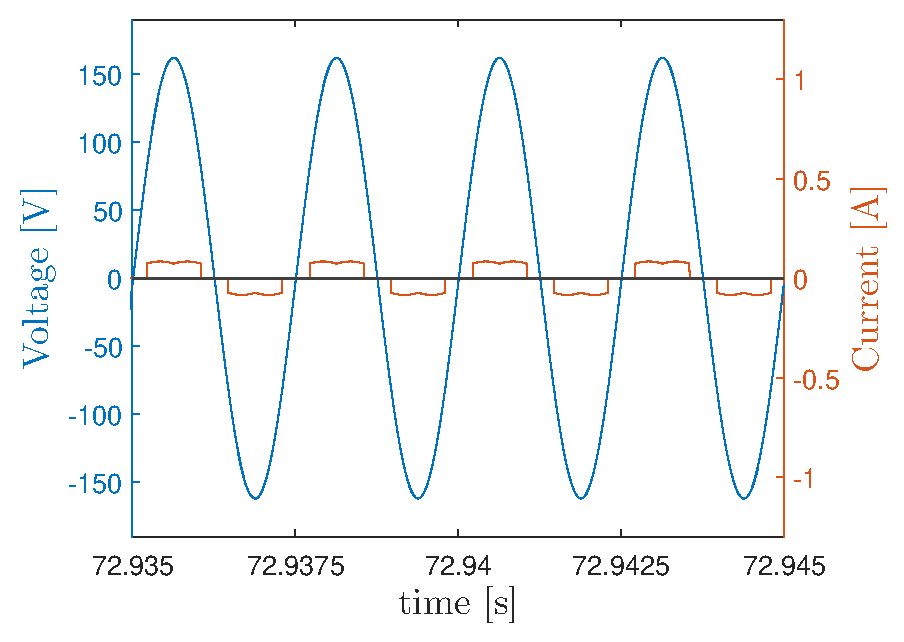
\includegraphics[width=0.27\textheight]{Figures/artigo_unfilt_1.eps}
	\caption{Voltage and current waveforms for the system without load and filter}
	\label{fig:artigo_unfilt_1.eps}
\end{figure}

\begin{figure}[!h] %
	\centering
	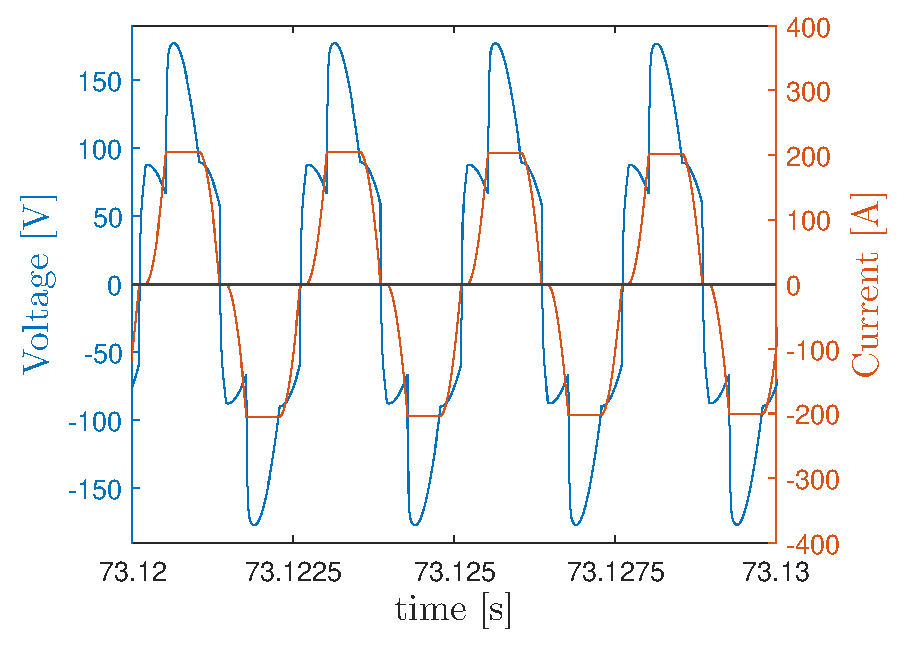
\includegraphics[width=0.27\textheight]{Figures/artigo_unfilt_2.eps}
	\caption{Voltage spectrum for the system without load and filter}
	\label{fig:artigo_unfilt_2.eps}
\end{figure}

\begin{figure}[!h] %
	\centering
	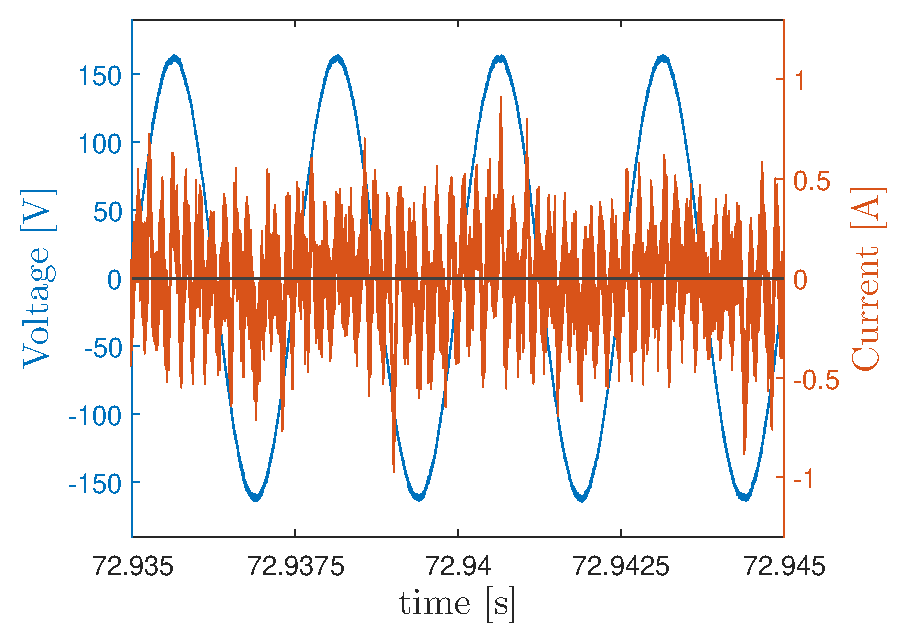
\includegraphics[width=0.27\textheight]{Figures/artigo_filt_1.eps}
	\caption{Voltage and current waveforms for the system without load and with filter}
	\label{fig:artigo_filt_1.eps}
\end{figure}

\begin{figure}[!h] %
	\centering
	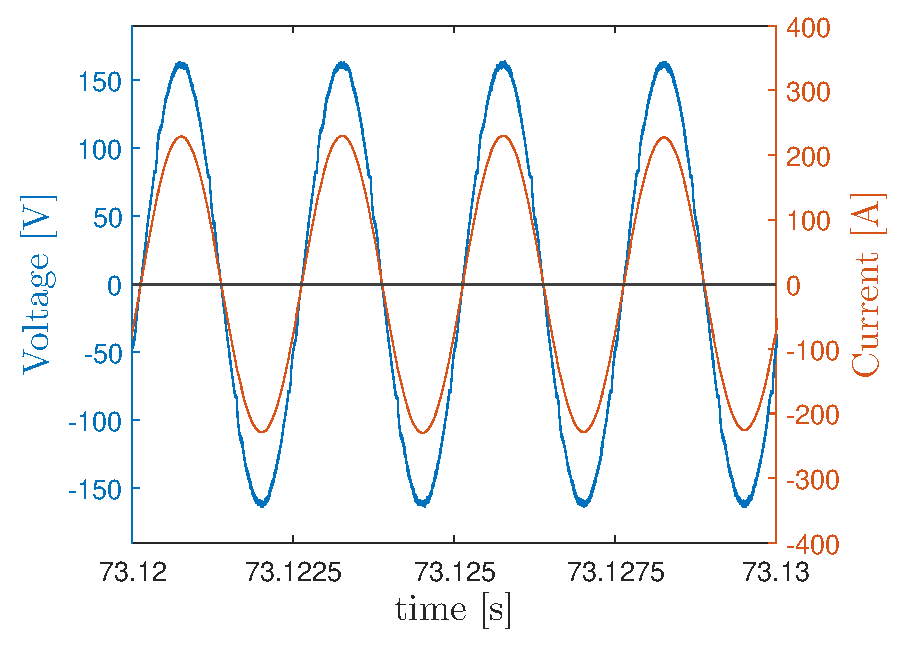
\includegraphics[width=0.27\textheight]{Figures/artigo_filt_2.eps}
	\caption{Voltage spectrum for the system without load and with filter}
	\label{fig:artigo_filt_2.eps}
\end{figure}

\begin{figure}[!h] %
	\centering
	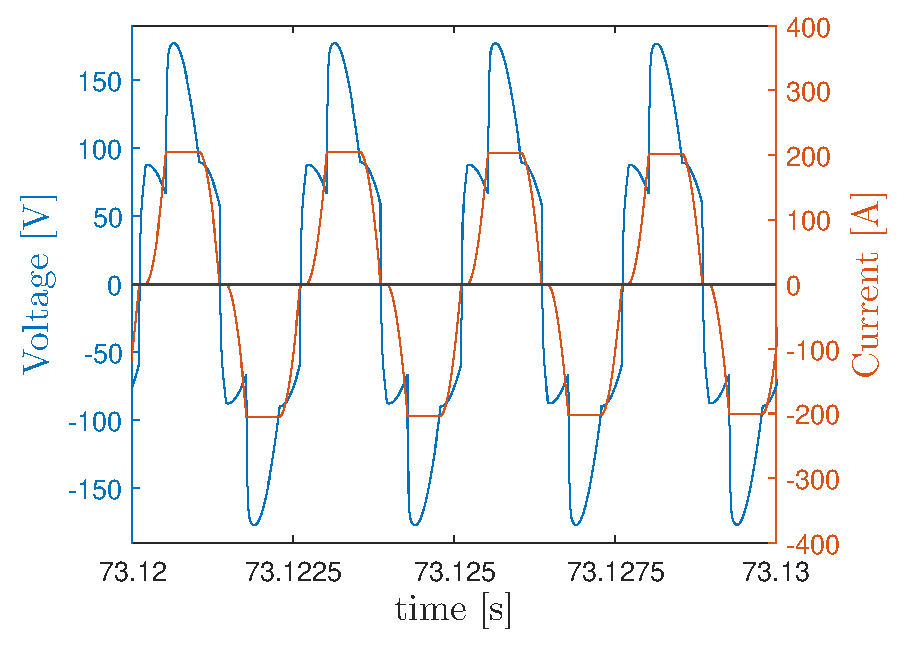
\includegraphics[width=0.27\textheight]{Figures/artigo_unfilt_3.eps}
	\caption{Voltage and current waveforms for the system with load and without filter}
	\label{fig:artigo_unfilt_3.eps}
\end{figure}

\begin{figure}[!h] %
	\centering
	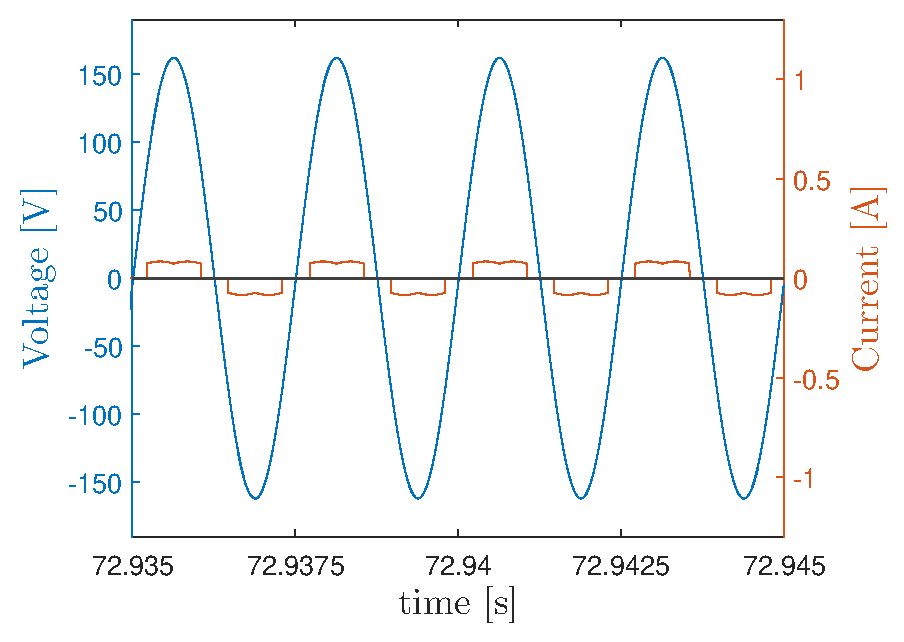
\includegraphics[width=0.27\textheight]{Figures/artigo_unfilt_4.eps}
	\caption{Voltage spectrum for the system with load and without filter}
	\label{fig:artigo_unfilt_4.eps}
\end{figure}

\begin{figure}[!h] %
	\centering
	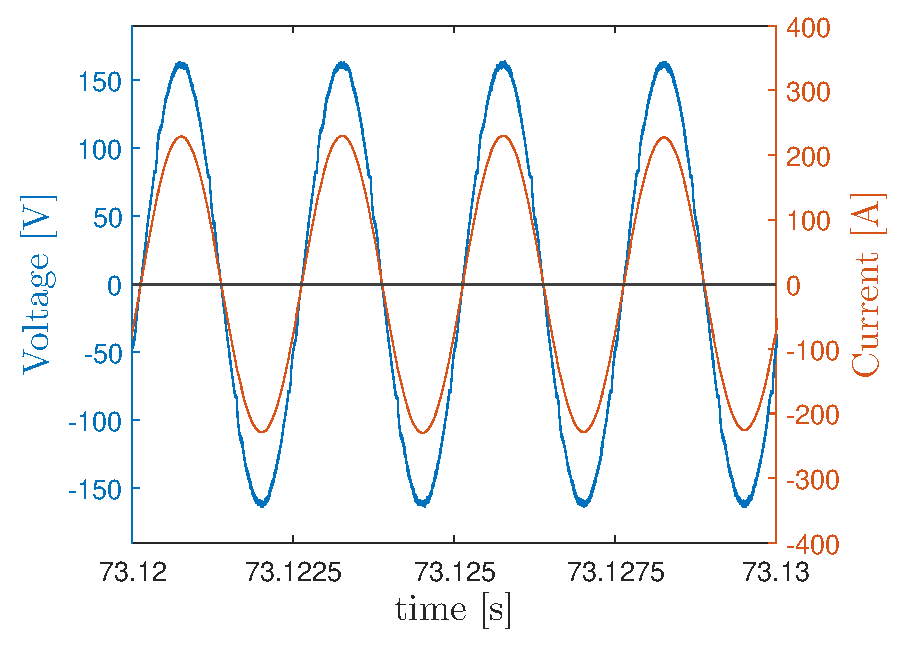
\includegraphics[width=0.27\textheight]{Figures/artigo_filt_3.eps}
	\caption{Voltage and current waveforms for the system with load and filter}
	\label{fig:artigo_filt_3.eps}
\end{figure}

\begin{figure}[!h] %
	\centering
	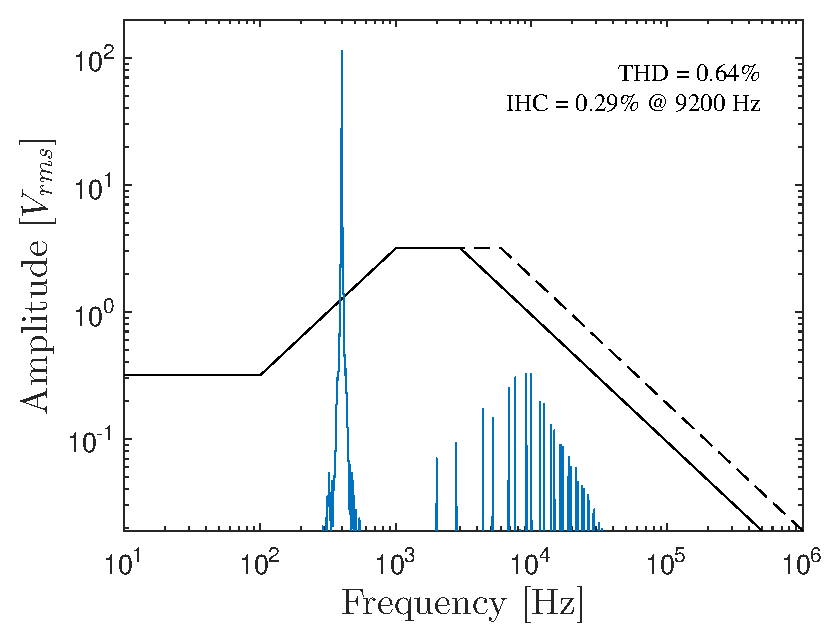
\includegraphics[width=0.27\textheight]{Figures/artigo_filt_4.eps}
	\caption{Voltage spectrum for the system with load and filter}
	\label{fig:artigo_filt_4.eps}
\end{figure}
